%mainfile: ../../master.tex
\subsection{Ultrasonic Sensor}\label{sub:ultrasonic}
The are number of different sensors for different purposes, depending on the purpose, they are based on following physical principles:
\begin{itemize}
  \item time of flight - for measuring a distance, thickness or integrity\cite{ultrasound2}
  \item the Doppler effect - for measuring speed\cite{ultrasound}
  \item the attenuation of sound waves - for measuring distance or directionality\cite{ultrasound}
\end{itemize}
The sensor HC-SR04 in consideration is utilizing time of flight principle. This sensor emit out a high-frequency (40 kHz) pulse, it then measures the time it takes for an echo of the pulse to reflect back. The sensor has 2 openings on its front. One opening emits ultrasonic waves, it acts as a speaker, a transmitter, the other receives them, acts as a microphone, a receiver.

\paragraph{The technology}
Ultrasonic soundwaves is at frequencies above human auditorial capablity, often at 40 kHz. Ultrasonic sound has a number of properties, relative to human audible sound, that can be exploited when in need of measuring the speed\cite{ultrasound}, thickness\cite{ultrasound2}, integrity\cite{ultrasound2} of an object, but also a distance to object as will be usefull in this context. These properties include the attenuation and reflectiveness of higher frequency waves and not being audible to humans.\chnote{more?} The sensors utilising this technology are very usefull for making measurements without touching or otherwise impeding a target. However, these following factors has to be taking into consideration in that may affect measurements.
  \subparagraph{Considerations}\label{sup:cons}
  \begin{itemize}
  \item Temperatures and humidity affect the speed of sound in air
  \item Temperature variations and air currents can act as invisible boundaries that will reflect ultrasonic waves
  \item The angle of the objects being observed. For the transmitted wave to echoed back to the receiver, the surface of the target must be  near perpendicular to the transmitter. Therfore the angle of the object with respect to the sensor does not exceed a particular range
  \item Pulsing ultrasonic sensors may have a “dead zone” immediately in front of them, in which objects will be detected correctly because they may reflect the wave before the receiver is operational, to avoid reverberations
  \item Some materials may be more absorbent than others, and will therefore reflect less ultrasonic waves
  \end{itemize}

\paragraph{The purpose} of the ultrasonic sensor in this project is figure out if a person is at a specific location in the problem domain eg. sitting in the sofa watching tv, where the PIR sensor\cref{sub:pir} is only capable of the measuring changes in infrared light over a larger(>100 degrees)\chnote{change to real values} angle, this sensor is capable of measuring a distance to an specifc object eg. a person. The distance is measured every second, so where is the PIR sensor\cref{sub:pir} would not capable of tracking a person if the person is not moving, the ultrasonic can detect a person by a change in distance from static state.

\paragraph{The tests} of the sensors will include some aspects of the considerations\cref{sup:cons} mentioned above, also some tests on the values mentioned in the HC-SR04 datasheet\cite{hcsr04}.
  
  \subparagraph{Distance}
  min and max distance, Error over different distances
  \chnote{sæt ind}
    \begin{figure}[htbp]
    \centering
    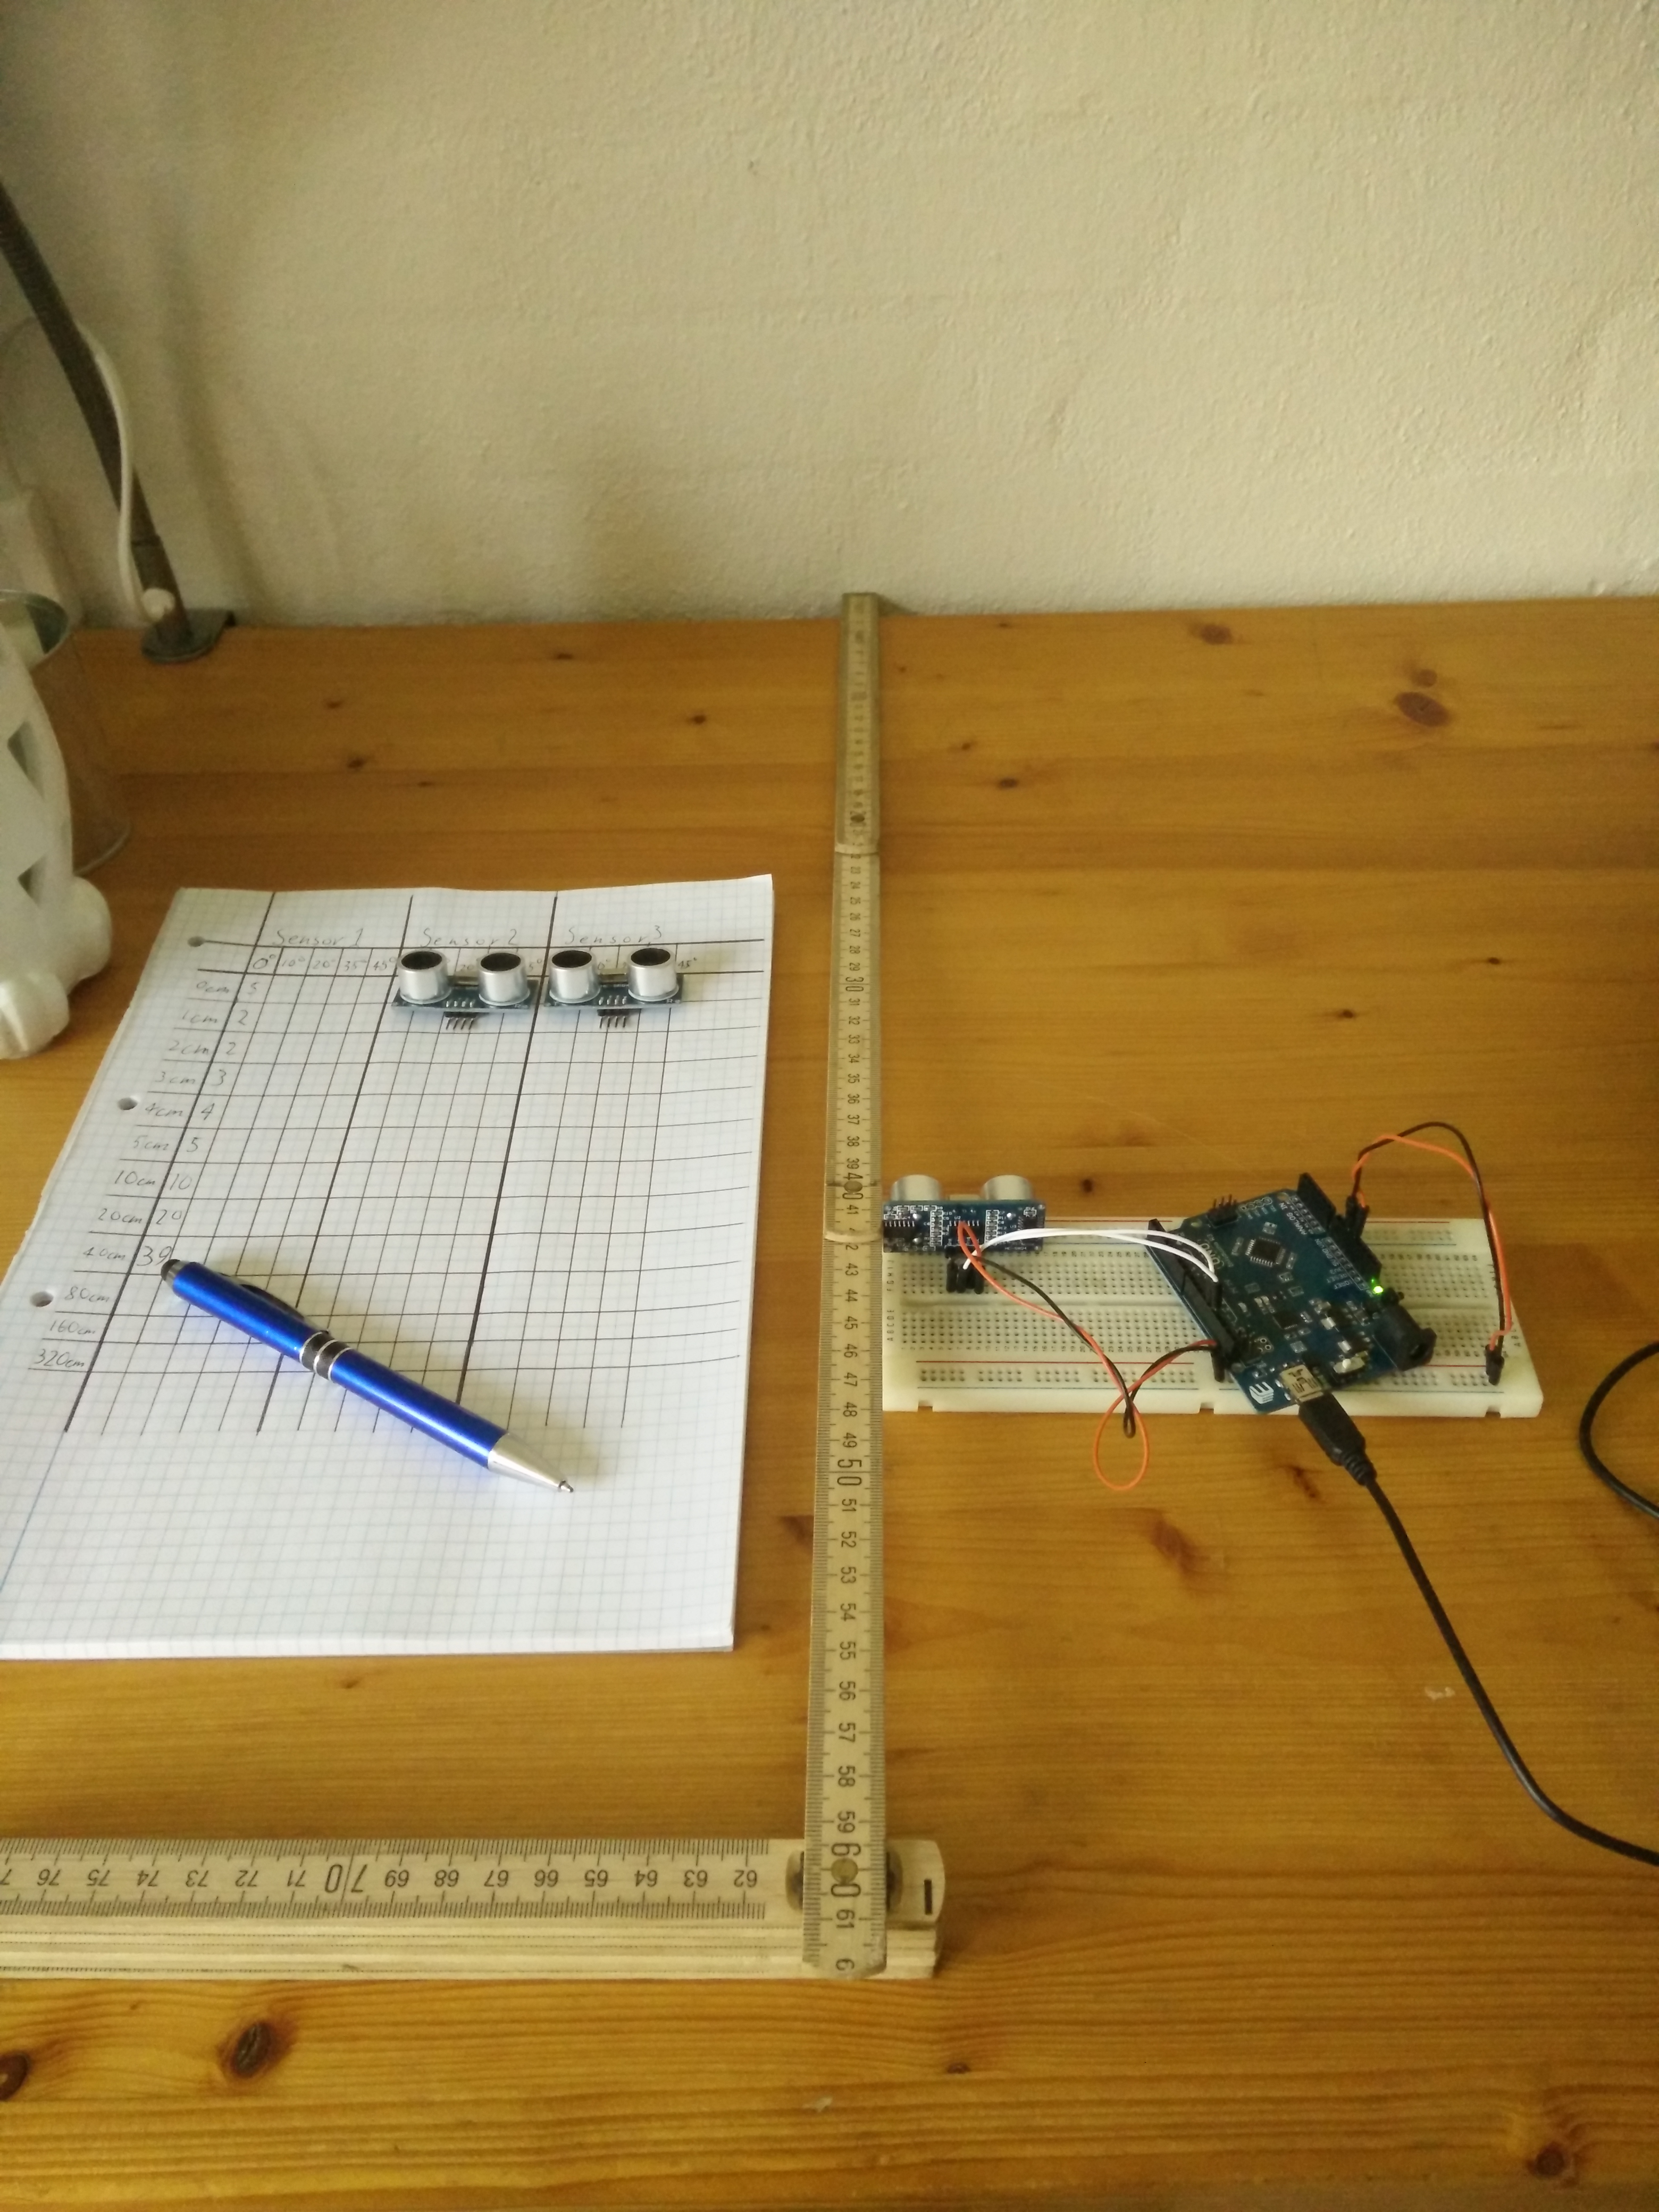
\includegraphics[width=\textwidth]{ultra1.jpg}
    \caption{bla}
    \label{fig:ultra1}
  \end{figure}
    \begin{figure}[htbp]
    \centering
    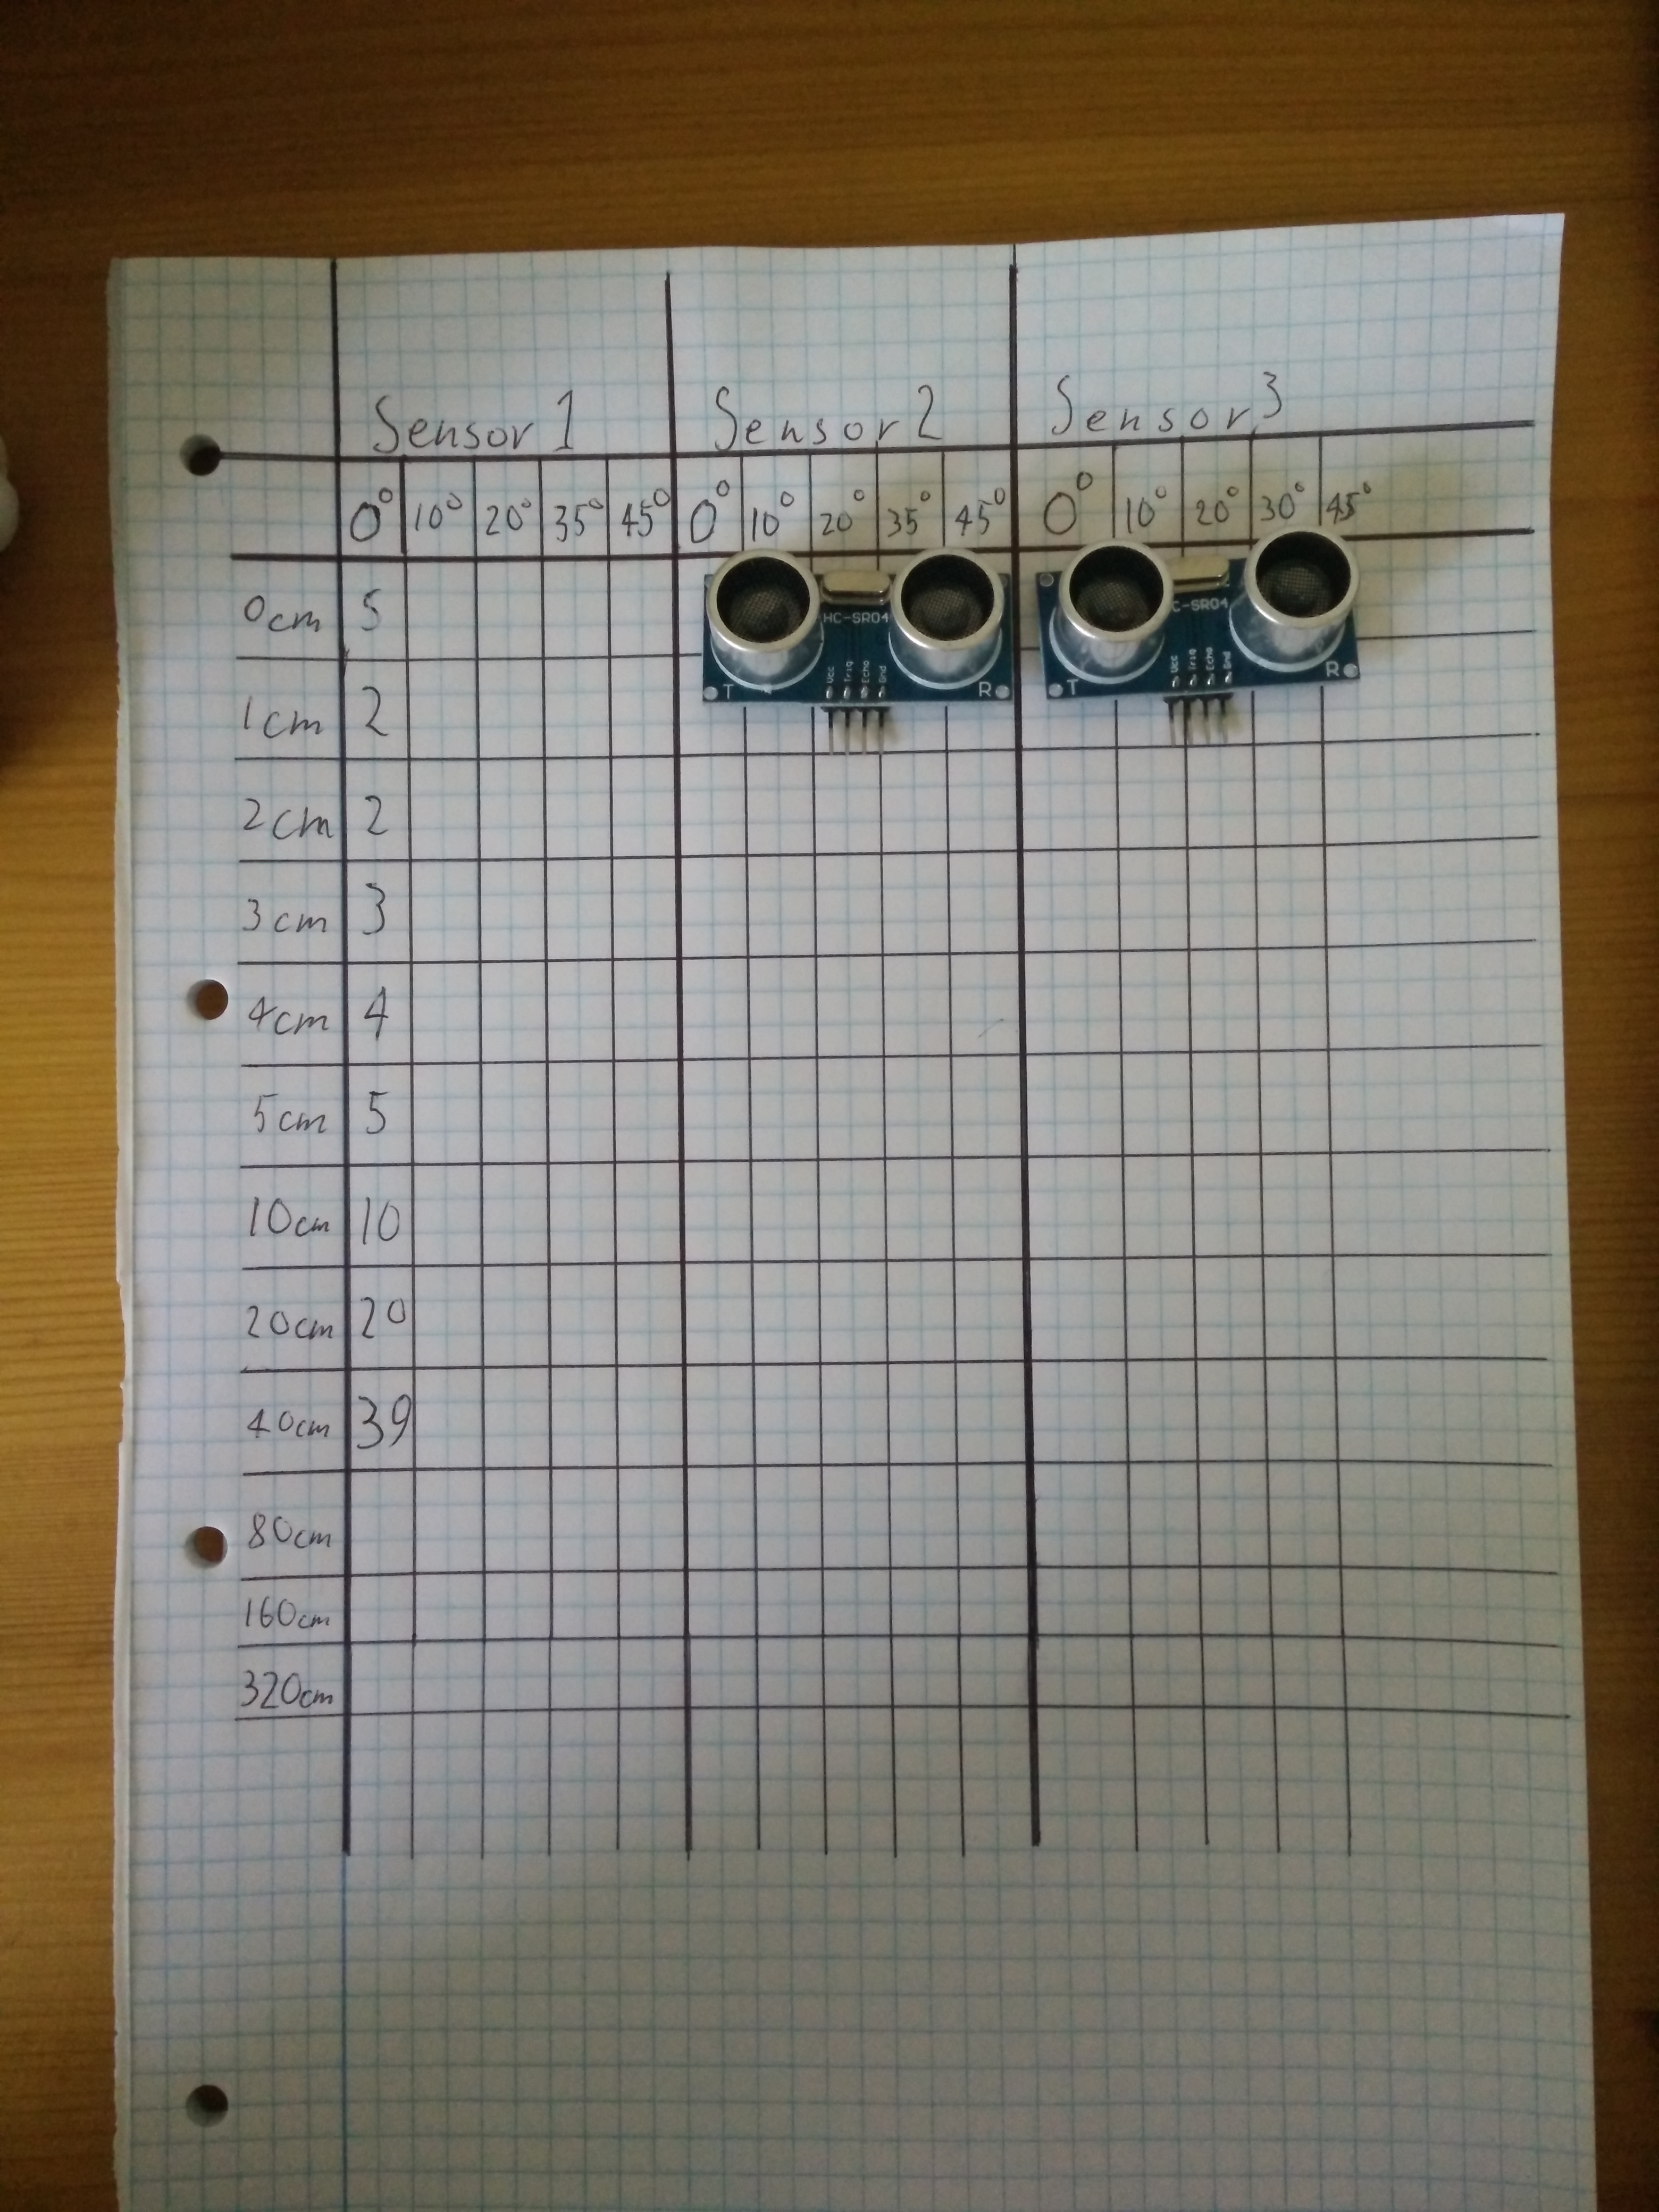
\includegraphics[width=\textwidth]{ultra2.jpg}
    \caption{bla}
    \label{fig:ultra2}
  \end{figure}
  \subparagraph{Angles}
  Of object, Of sensor
  \chnote{sæt ind}
  \begin{figure}[htbp]
    \centering
    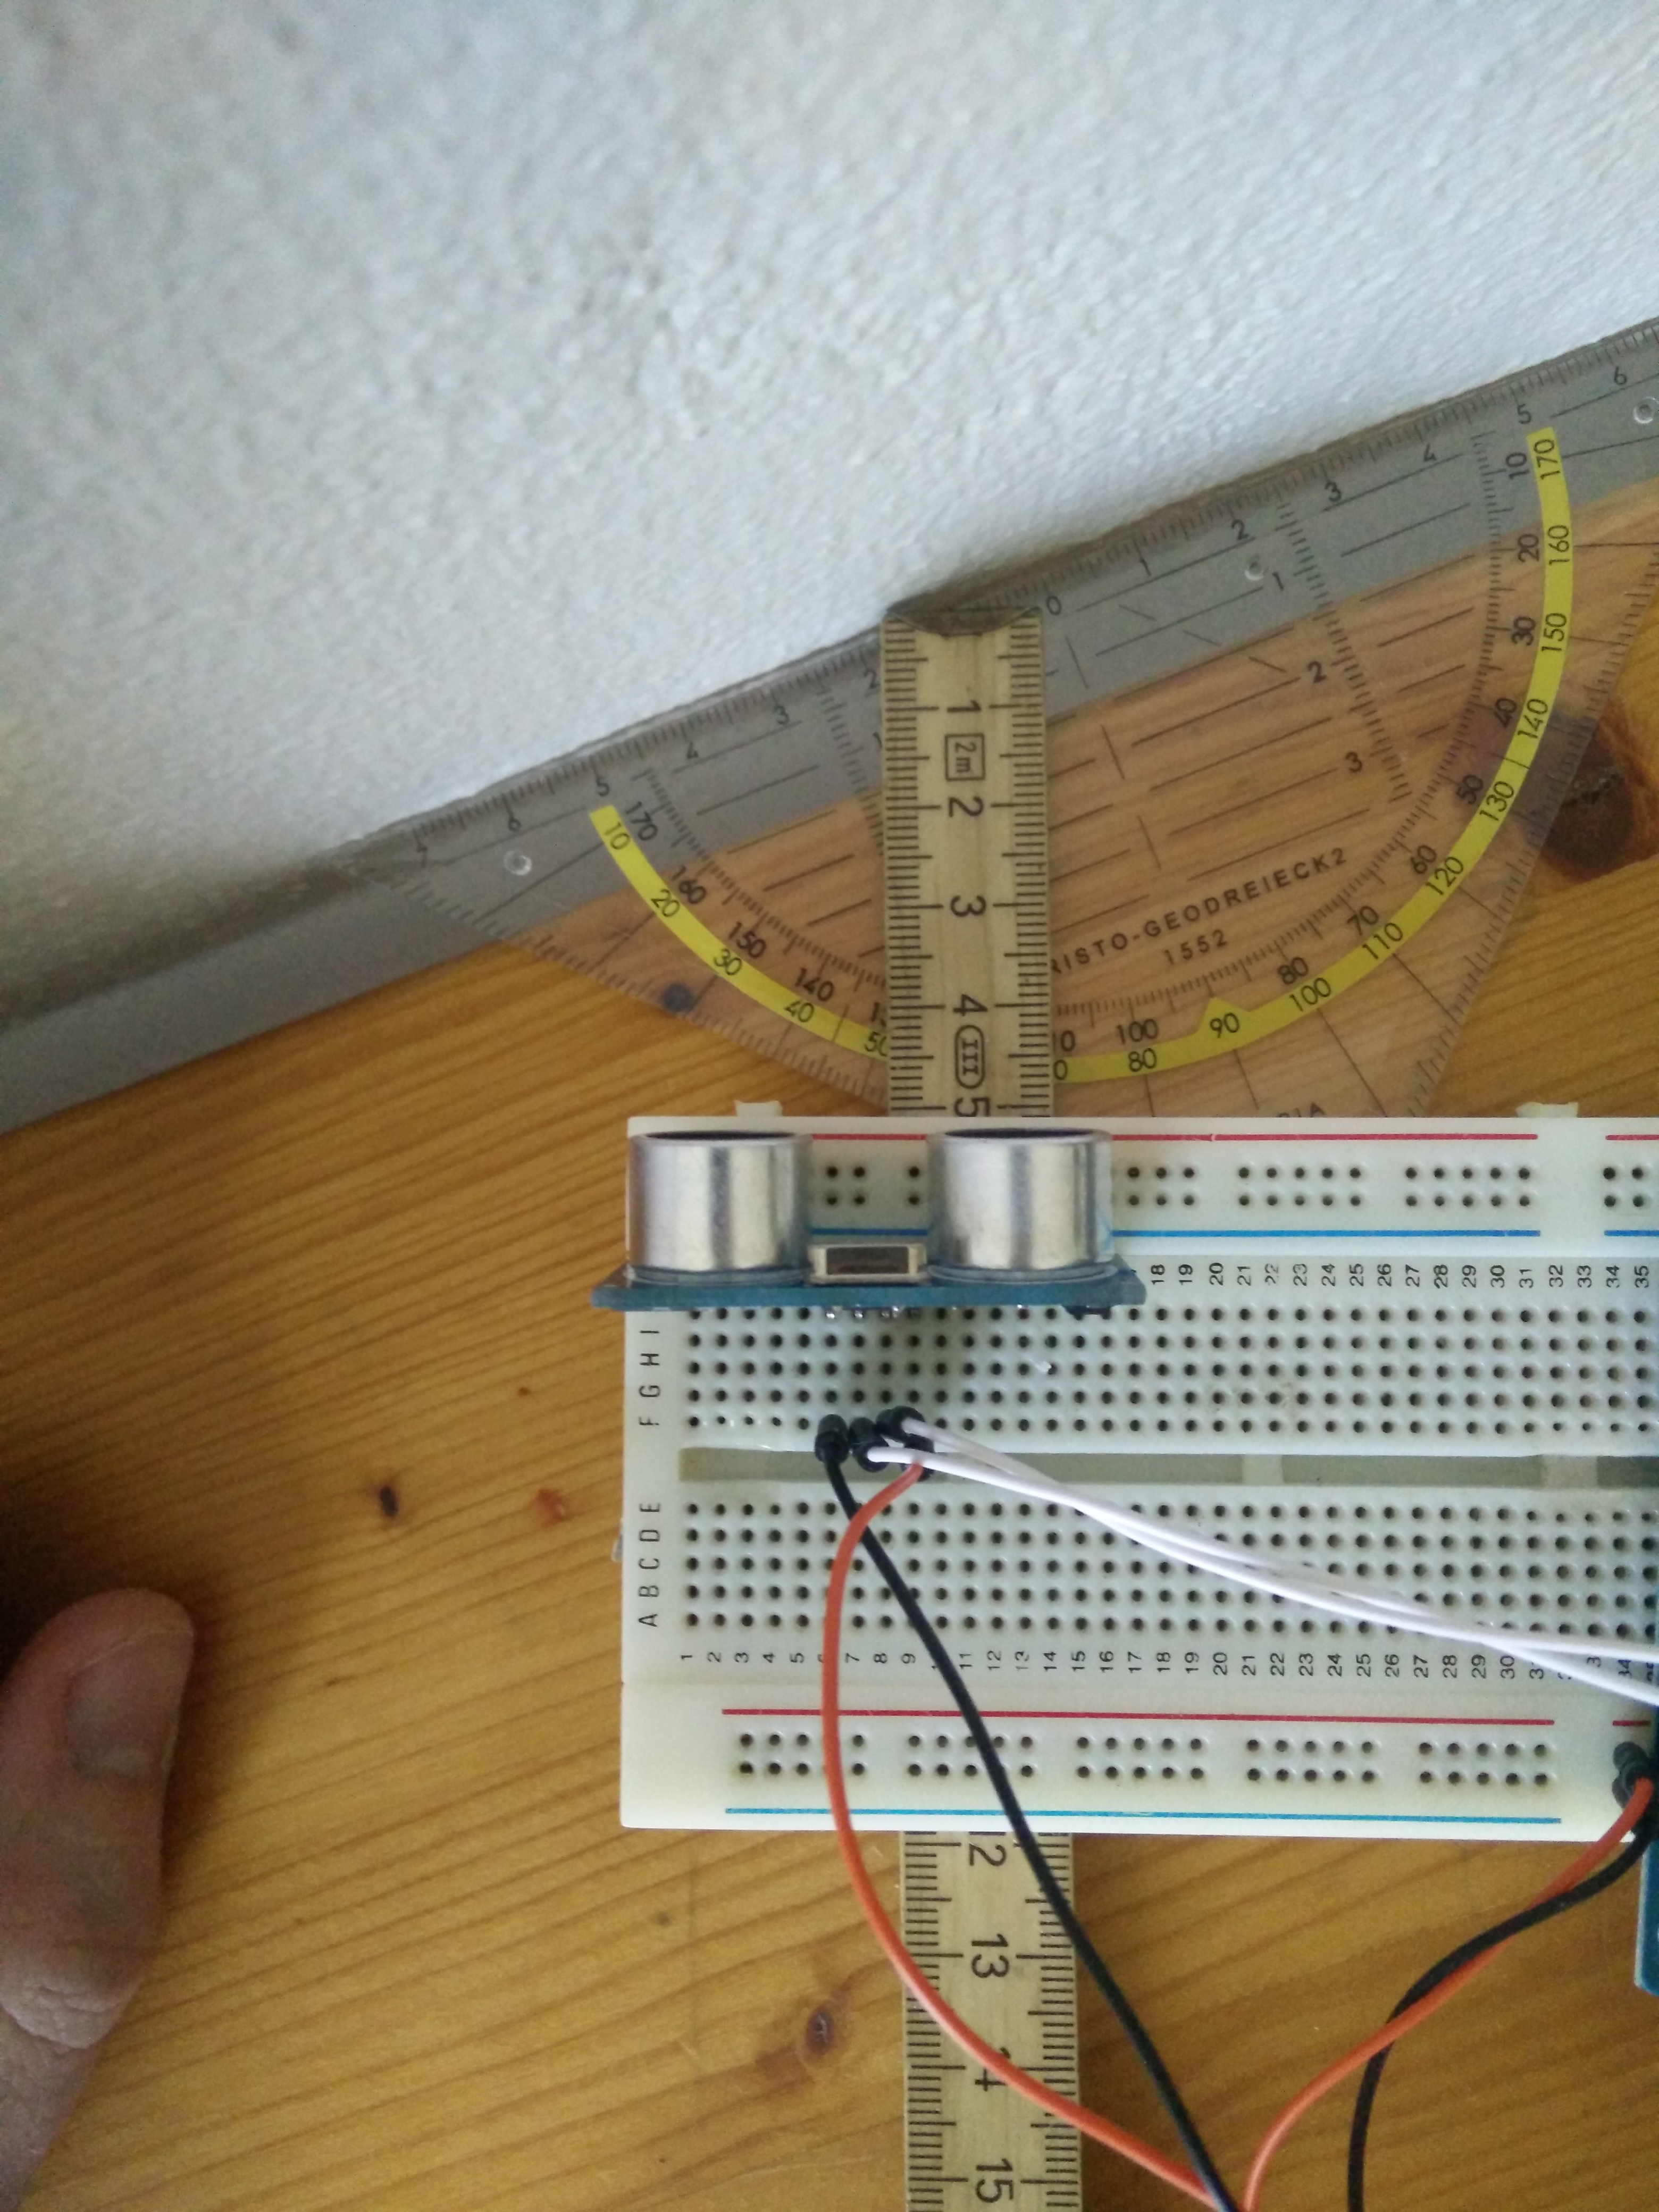
\includegraphics[width=\textwidth]{ultra3.jpg}
    \caption{bla}
    \label{fig:ultra3}
  \end{figure}
  
\paragraph{Multiple ultrasonic sensors} in the problem domain may introduction interference in the measurements performed, in that if one sensor is capable of transmitting soundwaves to another sensor it is possible that this will result in a collision. If this is to be solved it is important that a collision is detectable or does simply not happen. Getting collision free measurements requires some coordination between sensors, who will talk when. Example of a solution, each sensor is given a timeslot, in which a sensor is allowed to speak, it is important that theres is slight delay between each timeslot to ensure that the sounds wave has attenuated.\chnote{måske noget om dynamisk kunne tilslutte frakoble sensors}
